\chapter{Metabolismo microbiano y biopelículas}\label{ch:b2:microbial-metabolism}

Llénese un cilindro de vidrio con barro de charca, un poco de papel
triturado, una yema de huevo y agua, y déjese en el alféizar de una
ventana. En pocas semanas se estratifica en bandas de colores: algas
verdes arriba, una capa herrumbrosa, una banda púrpura, otra verde más
abajo y barro negro de sulfuro en el fondo. No se ha añadido nada más que
luz. Cada banda es una población que vive de una química distinta --- del
oxígeno, del nitrato, del sulfato, del sulfuro, del hidrógeno --- y cada
una alimenta a la siguiente. La columna es el mundo microbiano en
miniatura: células que obtienen su energía de casi cualquier par de
sustancias capaces de intercambiar electrones y que, en conjunto, hacen
funcionar los ciclos químicos del planeta. Este capítulo expone la lógica
de esa energética, la cinética del crecimiento microbiano y la vida
colectiva de los microbios sobre superficies, que es como vive realmente
la mayoría de ellos.

\section{Maneras de ganarse la vida}

\begin{definition}[Tipos tróficos]\label{def:b2:microbial-metabolism:trophic}
\index{quimiótrofo}\index{fotótrofo}\index{litótrofo}\index{organótrofo}
Un organismo se clasifica según tres respuestas. Su \emph{fuente de energía}:
la luz (\emph{fotótrofo}) o reacciones químicas (\emph{quimiótrofo}).
Su \emph{fuente de electrones}: sustancias inorgánicas --- $\mathrm{H_2}$,
$\mathrm{H_2S}$, $\mathrm{NH_4^+}$, $\mathrm{Fe^{2+}}$, el agua ---
(\emph{litótrofo}) o moléculas orgánicas (\emph{organótrofo}). Su
\emph{fuente de carbono}: el $\mathrm{CO_2}$ (\emph{autótrofo}) o el
carbono orgánico (\emph{heterótrofo}). Las plantas y las cianobacterias
son fotolitoautótrofas; los animales, los hongos y \emph{E.~coli} son
quimioorganoheterótrofos; las bacterias nitrificantes y las oxidantes
del azufre son quimiolitoautótrofas: fabrican su materia orgánica a
partir del $\mathrm{CO_2}$ con la energía obtenida de la oxidación de
minerales, en la oscuridad. Casi todas las combinaciones existen en algún
\omterm{def:b2:unicellular-diversity:prokaryote}{procariota}; los eucariotas solo ocupan dos.
\end{definition}

\begin{theorem}[La energía de un par redox]\label{thm:b2:microbial-metabolism:redox}
\index{potencial redox}\index{torre de electrones}
Todo metabolismo productor de energía transfiere electrones de un par
\emph{dador} a un par \emph{aceptor}. Cada par tiene un potencial estándar
$E^{\circ\prime}$ (a pH 7): cuanto más negativo, más fácilmente cede
electrones. Transferir $n$ moles de electrones de un dador a $E_d$ a un
aceptor a $E_a$ libera una energía libre estándar
\[
\Delta G^{\circ\prime} = -\,n F\,(E_a - E_d), \qquad F = \qty{96.5}{kJ/V/mol},
\]
de modo que el rendimiento es proporcional a la distancia vertical entre
los dos pares en la \emph{\omterm{thm:b2:microbial-metabolism:redox}{torre de electrones}}. Con
$\mathrm{O_2/H_2O}$ a \qty{+0.82}{V} y $\mathrm{CO_2}$/glucosa a
\qty{-0.43}{V}, los 24 electrones de una molécula de glucosa rinden
$24\times 96.5\times 1.25 = \qty{2900}{kJ/mol}$; cedidos en cambio al
sulfato ($\mathrm{SO_4^{2-}/H_2S}$, \qty{-0.22}{V}), los mismos
electrones solo rinden $24\times 96.5\times 0.21 = \qty{490}{kJ/mol}$.
\end{theorem}
\begin{proof}
Para la reacción dador$_{\text{red}}$ + aceptor$_{\text{ox}}$
$\to$ dador$_{\text{ox}}$ + aceptor$_{\text{red}}$, la variación de energía
libre es el trabajo realizado por $n$ moles de carga electrónica $nF$ al
caer a través de la diferencia de potencial $E_a - E_d$, con el convenio
de signos según el cual una transferencia espontánea (electrones hacia el
par más positivo) tiene $\Delta G < 0$. Es la relación de Nernst del
volumen del primer año aplicada a dos semirreacciones.
\end{proof}

\begin{omfigure}
\begin{tikzpicture}[every node/.style={font=\scriptsize}, y=6cm]
  \draw[thick, ->] (0,-0.55) -- (0,0.95) node[above] {$E^{\circ\prime}$ (V)};
  \foreach \v in {-0.4,-0.2,0,0.2,0.4,0.6,0.8} \draw (-0.08,\v) -- (0.08,\v) node[right, xshift=0.05cm] {\v};
  % donors on the right: value/label position/text
  \foreach \v/\y/\l in {-0.43/-0.49/{$\mathrm{CO_2}$/glucosa}, -0.42/-0.40/{$2\mathrm{H^+/H_2}$}, -0.32/-0.31/{$\mathrm{NAD^+/NADH}$}, -0.27/-0.22/{$\mathrm{S^0/H_2S}$}, 0.03/0.03/{fumarato/succinato}, 0.34/0.34/{$\mathrm{NO_2^-/NH_4^+}$}}
    { \draw[omDef, thick] (0.8,\v) -- (1.6,\v); \draw[omDef] (1.6,\v) -- (1.85,\y); \node[omDef, anchor=west] at (1.9,\y) {\l}; }
  % acceptors on the left
  \foreach \v/\y/\l in {-0.24/-0.29/{$\mathrm{CO_2/CH_4}$}, -0.22/-0.17/{$\mathrm{SO_4^{2-}/H_2S}$}, 0.43/0.43/{$\mathrm{NO_3^-/NO_2^-}$}, 0.74/0.69/{$\mathrm{NO_3^-/N_2}$}, 0.77/0.77/{$\mathrm{Fe^{3+}/Fe^{2+}}$}, 0.82/0.86/{$\mathrm{O_2/H_2O}$}}
    { \draw[omThm, thick] (-1.6,\v) -- (-0.8,\v); \draw[omThm] (-1.6,\v) -- (-1.85,\y); \node[omThm, anchor=east] at (-1.9,\y) {\l}; }
  \node[omThm, anchor=south] at (-2.4,0.93) {aceptores};
  \node[omDef, anchor=south] at (2.4,0.93) {dadores};
  % arrows showing two metabolisms
  \draw[->, very thick, omExo!80!black] (4.9,-0.43) -- (4.9,0.80);
  \node[anchor=west, align=left] at (5.0,0.2) {respiración aerobia\\de la glucosa: \qty{1.25}{V},\\\qty{2900}{kJ/mol}};
  \draw[->, very thick, omProp] (4.2,-0.43) -- (4.2,-0.24);
  \node[anchor=north, align=center] at (4.2,-0.52) {reducción del sulfato:\\\qty{0.21}{V}, \qty{490}{kJ/mol}};
  \draw[dashed, gray] (3.5,-0.43) -- (4.9,-0.43);
  \draw[dashed, gray] (3.5,0.82) -- (4.9,0.82);
  \draw[dashed, gray] (3.5,-0.22) -- (4.2,-0.22);
\end{tikzpicture}

{\small La \omterm{thm:b2:microbial-metabolism:redox}{torre de electrones}. Los dadores (azul) se sitúan en sus
potenciales estándar, y los aceptores (rojo) igualmente. Un metabolismo
es una caída desde un dador hasta un aceptor situado por encima, y su
rendimiento energético es proporcional a la altura de la caída: de la
glucosa al oxígeno la caída es larga; de la glucosa al sulfato, corta.}
\end{omfigure}

\begin{proposition}[Quimiolitotrofia]\label{prop:b2:microbial-metabolism:lithotrophy}
\index{quimiolitotrofia}\index{nitrificación}
Algunas bacterias obtienen toda su energía de oxidaciones inorgánicas,
con el oxígeno (o el nitrato) como aceptor, y fijan el $\mathrm{CO_2}$
con el ATP y el poder reductor así obtenidos. \emph{Nitrificantes}: las
oxidantes del amonio (\emph{Nitrosomonas}) transforman el
$\mathrm{NH_4^+}$ en nitrito ($\Delta G^{\circ\prime} = \qty{-275}{kJ/mol}$),
y las oxidantes del nitrito (\emph{Nitrobacter}) transforman el nitrito
en nitrato (\qty{-74}{kJ/mol}); juntas convierten el amonio de la
descomposición en el nitrato que absorben las plantas
(\cref{ch:b2:biogeochemical-cycles}).
\emph{Oxidantes del azufre} (\emph{Thiobacillus}, \emph{Beggiatoa}):
oxidan el $\mathrm{H_2S}$ a azufre y sulfato; las \emph{oxidantes del
hierro} oxidan el $\mathrm{Fe^{2+}}$ a herrumbre; las \emph{oxidantes
del hidrógeno} queman $\mathrm{H_2}$. Como sus dadores de electrones
están arriba en la torre, el rendimiento por molécula es pequeño, y como
sus dadores son reductores más débiles que el NADH, deben gastar energía
para impulsar electrones \emph{cuesta arriba} y fabricar el NADH que
necesita la fijación del carbono: una nitrificante oxida unos treinta
iones amonio para fijar un $\mathrm{CO_2}$, y crece despacio.
\end{proposition}
\begin{proof}[Evidencia]
Winogradsky (1887--1890) cultivó bacterias filamentosas del azufre en una
gota de agua en la que dejaba difundir sulfuro por un lado y aire por el
otro: se reunían en la frontera, acumulaban glóbulos de azufre y los
consumían cuando se cortaba el sulfuro. Después aisló bacterias
nitrificantes en un medio puramente mineral, con amonio y sin carbono
orgánico alguno, en el que crecían y producían nitrato --- la primera
demostración de que la vida puede construirse a partir del
$\mathrm{CO_2}$ y de la energía de una reacción inorgánica, sin luz. Lo
llamó quimiosíntesis.
\end{proof}

\begin{omfigure}
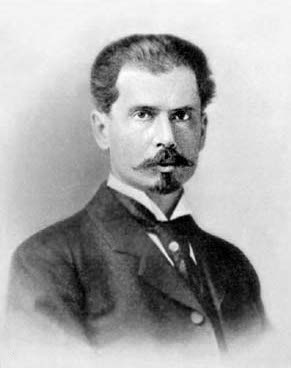
\includegraphics[width=0.26\linewidth]{images/book4/winogradsky.jpg}\hspace{0.05\linewidth}
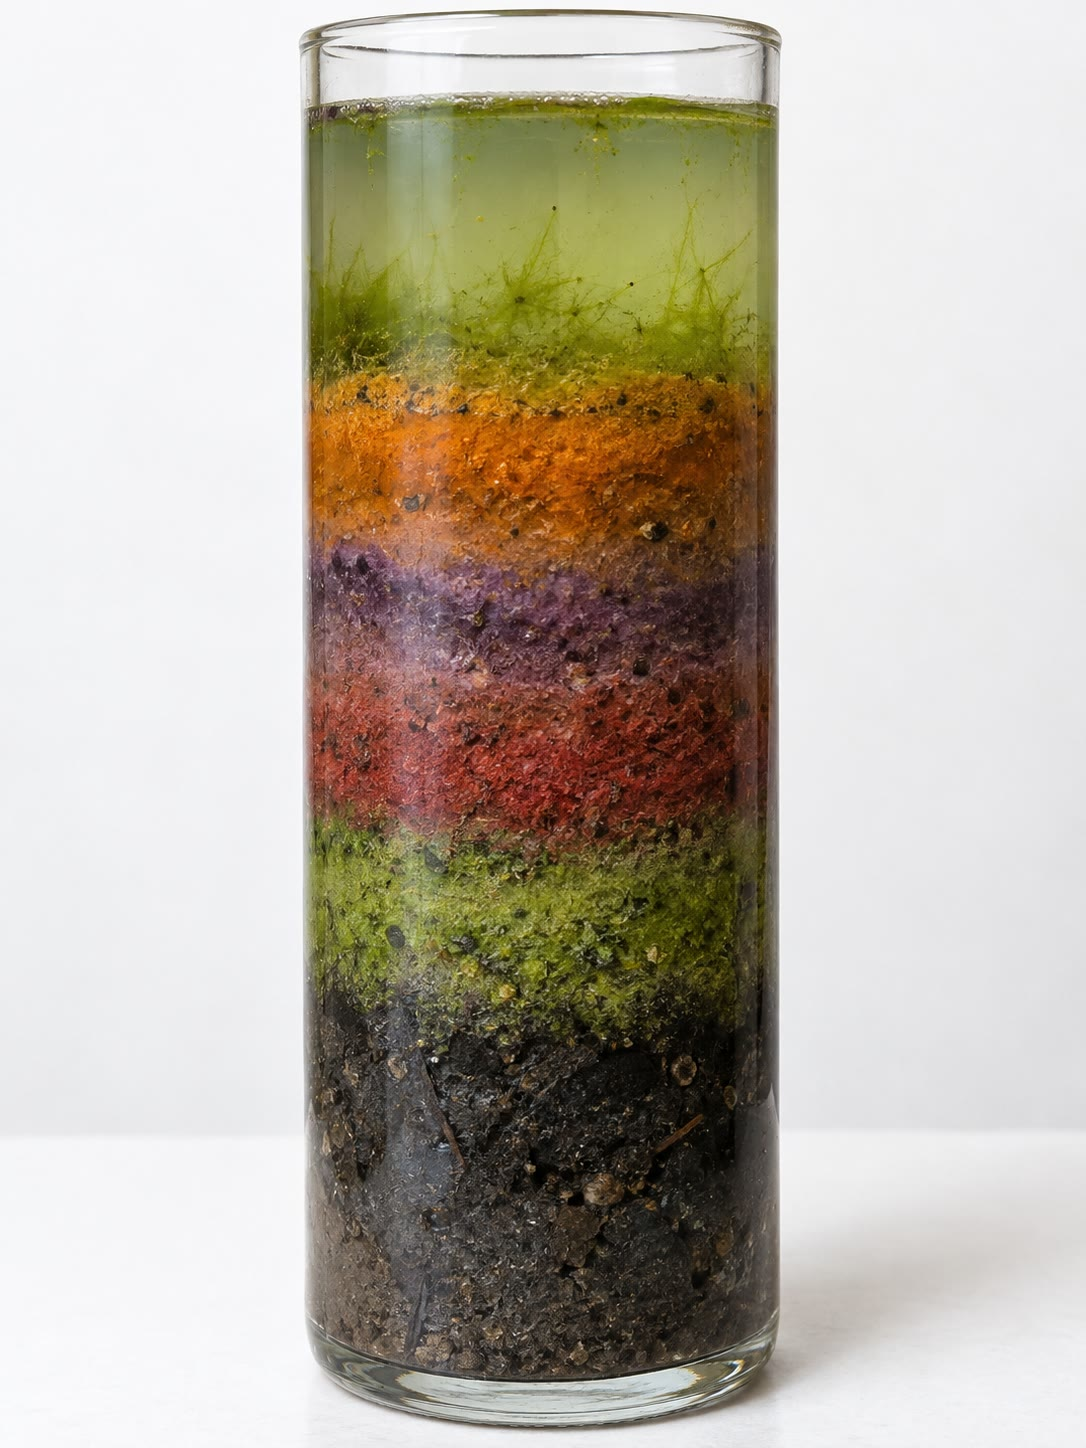
\includegraphics[width=0.30\linewidth]{images/book4/ai/b4-02-winogradsky-column.jpg}

{\small Serguéi Winogradsky, que descubrió la \omterm{def:b2:microbial-metabolism:trophic}{quimiolitotrofia}, y la
columna que lleva su nombre: un cilindro de barro y agua que, a la luz,
se estratifica en bandas de algas, oxidantes del hierro y del azufre,
bacterias púrpuras y verdes del azufre, y reductoras del sulfato en el
barro negro.}
\end{omfigure}

\begin{definition}[Fotosíntesis anoxigénica]\label{def:b2:microbial-metabolism:anoxygenic}
\index{fotosíntesis anoxigénica}
Las bacterias púrpuras y verdes realizan la fotosíntesis con un solo
fotosistema y una bacterioclorofila que absorbe en el infrarrojo
cercano, y usan $\mathrm{H_2S}$, $\mathrm{H_2}$ o ácidos orgánicos como
dadores de electrones en lugar del agua: liberan azufre o sulfato, nunca
oxígeno, y necesitan luz de longitudes de onda que atraviesen la capa de
algas verdes y cianobacterias situada por encima. Por eso las bacterias
púrpuras del azufre crecen en la banda púrpura de la columna de
Winogradsky, justo donde el sulfuro que sube del fondo se encuentra con
la luz que llega desde arriba; las bacterias verdes del azufre, que
toleran más sulfuro y menos luz, crecen debajo de ellas. La fotosíntesis
oxigénica, con sus dos fotosistemas en serie, es una invención posterior
de un solo linaje --- las cianobacterias --- que aprendió a tomar
electrones del agua.
\end{definition}

\section{Respiraciones anaerobias y fermentaciones}

\begin{definition}[Respiración anaerobia]\label{def:b2:microbial-metabolism:anaerobic}
\index{respiración anaerobia}\index{desnitrificación}\index{reducción del sulfato}\index{metanogénesis}
La \emph{respiración anaerobia} es una respiración --- una cadena de
transporte de electrones que bombea protones y fabrica ATP por
quimiósmosis --- con un aceptor final distinto del oxígeno. Las
\emph{desnitrificantes} (\emph{Pseudomonas}, \emph{Paracoccus}) reducen
el nitrato a nitrito, óxido nítrico, óxido nitroso y finalmente
$\mathrm{N_2}$, que escapa a la atmósfera; usan su cadena aerobia con
unas pocas enzimas añadidas y solo pasan al nitrato cuando se ha agotado
el oxígeno. Las \emph{reductoras del sulfato} (\emph{Desulfovibrio})
reducen el sulfato a sulfuro, ennegrecen el barro con sulfuro de hierro y
le dan su olor. Los \emph{metanógenos}, que son arqueas, reducen el
$\mathrm{CO_2}$ con $\mathrm{H_2}$ a
metano ($4\mathrm{H_2} + \mathrm{CO_2} \to \mathrm{CH_4} +
2\mathrm{H_2O}$, $\Delta G^{\circ\prime} = \qty{-131}{kJ/mol}$), o
escinden el acetato en metano y $\mathrm{CO_2}$; el oxígeno los mata, y
viven en el rumen de las vacas, los arrozales, las marismas y los
vertederos, desde donde liberan un gas de efecto invernadero que es
objeto del \cref{ch:b2:global-change}. Los óxidos de hierro y de
manganeso sirven a otros grupos. El volumen del primer año trataba el
oxígeno como \emph{el} aceptor; durante la mayor parte de la historia de
la Tierra, y hoy en todo sedimento, es solo el primero de una serie.
\end{definition}

\begin{proposition}[La secuencia de aceptores en un sedimento]\label{prop:b2:microbial-metabolism:sequence}
Al descender por un sedimento encharcado, los aceptores de electrones se
agotan en el orden de la energía que rinden: el oxígeno en los primeros
milímetros, después el nitrato, luego los óxidos de manganeso y de hierro,
después el sulfato y, por último, el $\mathrm{CO_2}$ (\omterm{def:b2:microbial-metabolism:anaerobic}{metanogénesis}) en la
capa anóxica más profunda. El orden es el de la torre: a cada
profundidad, los organismos que usan el mejor aceptor restante crecen
más deprisa, desplazan a los demás en la competencia por los dadores
orgánicos y agotan su aceptor antes de que tome el relevo el grupo
siguiente. En el mar, donde el sulfato abunda (\qty{28}{mmol/L}), la zona
del sulfato es gruesa y la \omterm{def:b2:microbial-metabolism:anaerobic}{metanogénesis} solo empieza a varios metros de
profundidad; en una marisma de agua dulce, pobre en sulfato, el metano se
forma justo bajo la superficie.
\end{proposition}
\begin{omfigure}
\begin{tikzpicture}[every node/.style={font=\scriptsize}]
  \fill[omDef!8] (0,0) rectangle (4,0.6);
  \node at (2,0.3) {agua};
  \fill[omExo!35] (0,-0.5) rectangle (4,0);
  \fill[omProp!25] (0,-1.3) rectangle (4,-0.5);
  \fill[omProp!45] (0,-2.0) rectangle (4,-1.3);
  \fill[gray!50] (0,-3.4) rectangle (4,-2.0);
  \fill[black!75] (0,-4.4) rectangle (4,-3.4);
  \draw[thick] (0,0.6) -- (0,-4.4); \draw[thick] (4,0.6) -- (4,-4.4);
  \draw[thick] (0,0) -- (4,0);
  \node[anchor=west, align=left] at (4.2,-0.25) {respiración del oxígeno: $\mathrm{O_2 \to H_2O}$ --- \qty{2.9}{MJ} por glucosa};
  \node[anchor=west, align=left] at (4.2,-0.9) {reducción del nitrato: $\mathrm{NO_3^- \to N_2}$ --- \qty{2.7}{MJ}};
  \node[anchor=west, align=left] at (4.2,-1.65) {reducción del manganeso y del hierro: $\mathrm{Fe^{3+} \to Fe^{2+}}$};
  \node[anchor=west, align=left, white] at (0.1,-2.7) {};
  \node[anchor=west, align=left] at (4.2,-2.7) {reducción del sulfato: $\mathrm{SO_4^{2-} \to H_2S}$ --- \qty{0.5}{MJ}};
  \node[anchor=west, align=left] at (4.2,-3.9) {metanogénesis: $\mathrm{CO_2 \to CH_4}$ --- \qty{0.4}{MJ}};
  \draw[->, thick] (-0.5,0) -- (-0.5,-4.4) node[below] {profundidad};
  \node[anchor=east] at (-0.6,-0.25) {mm};
  \node[anchor=east] at (-0.6,-2.7) {de cm a m};
\end{tikzpicture}

{\small La sucesión de aceptores de electrones con la profundidad en un
sedimento, en el orden de la energía que cada uno rinde por glucosa. Los
organismos de cada zona desplazan a los de la siguiente en la competencia
por la materia orgánica hasta agotar su aceptor.}
\end{omfigure}

\begin{definition}[La fermentación, revisitada]\label{def:b2:microbial-metabolism:fermentation}
\index{fermentación!microbiana}
Una \emph{fermentación} no usa ningún aceptor externo: el sustrato
orgánico se escinde en un producto más oxidado y otro más reducido, el
ATP se fabrica solo por fosforilación a nivel de sustrato, y el NADH de
la glucólisis se reoxida reduciendo un metabolito. Las levaduras producen
etanol y $\mathrm{CO_2}$; las bacterias lácticas, lactato (yogur, chucrut,
músculos doloridos); \emph{E.~coli}, una mezcla de ácidos, etanol y gases;
los clostridios, butirato, butanol y acetona; las propionibacterias, el
propionato y el $\mathrm{CO_2}$ del queso emmental. El rendimiento es de
dos ATP por glucosa, frente a unos treinta por respiración, de modo que un
fermentador debe procesar quince veces más azúcar para el mismo
crecimiento, y sus productos --- ácidos, alcohol --- envenenan su propio
medio: las fermentaciones conservan los alimentos porque el fermentador
los vuelve inhabitables, también para sí mismo.
\end{definition}

\begin{example}[Sintrofia: vivir de lo que queda]\label{ex:b2:microbial-metabolism:syntrophy}
En un sedimento anóxico los fermentadores dejan tras de sí acetato,
propionato, butirato y $\mathrm{H_2}$. Oxidar el propionato a acetato y
$\mathrm{H_2}$ tiene una energía libre estándar \emph{positiva}
(\qty{+76}{kJ/mol}) y es imposible --- a menos que un metanógeno vecino
consuma el hidrógeno tan deprisa como se forma y mantenga su presión
parcial por debajo de \qty{1e-4}{atm}, valor al que la reacción se vuelve
exergónica. Ninguno de los dos socios puede crecer solo con propionato;
juntos lo convierten en metano. Esta \emph{transferencia de hidrógeno
entre especies} explica que la digestión anaerobia sea siempre obra de
un consorcio, y que la arquea y su socia bacteriana se encuentren a
menudo pegadas la una a la otra.
\end{example}

\section{Crecimiento sobre un sustrato}

\begin{theorem}[Ley de Monod]\label{thm:b2:microbial-metabolism:monod}
\index{ecuación de Monod}\index{coeficiente de rendimiento}
Una población que crece sobre un único sustrato limitante de
concentración $S$ tiene una tasa específica de crecimiento
\[
\mu = \mu_{\max}\,\frac{S}{K_s + S}, \qquad \frac{\mathrm{d}X}{\mathrm{d}t} = \mu X,
\]
donde $X$ es la concentración de biomasa, $\mu_{\max}$ la tasa máxima
(el inverso del \omterm{def:b2:unicellular-diversity:division}{tiempo de generación} más corto, dividido por $\ln 2$) y
$K_s$ la \emph{constante de semisaturación}, la concentración de
sustrato a la que el crecimiento va a media velocidad --- unos pocos
miligramos de glucosa por litro para \emph{E.~coli}. El sustrato se
consume en proporción al crecimiento, $\mathrm{d}S/\mathrm{d}t =
-\mu X/Y$, con $Y$ el \emph{rendimiento}: gramos de biomasa por gramo de
sustrato, alrededor de \num{0.5} para el crecimiento aerobio sobre azúcar
y de \num{0.1} para un fermentador.
\end{theorem}
\begin{proof}[Evidencia]
Monod (1942) cultivó \emph{E.~coli} en lotes con una serie de
concentraciones de glucosa y midió la tasa exponencial de cada uno: las
tasas aumentaban con la concentración y se saturaban, como una curva de
Michaelis--Menten, que es lo que cabe esperar si la tasa la fija un
sistema de captación saturable. La ley es empírica --- una célula tiene
miles de enzimas, no una ---, pero se ajusta a casi todo cultivo limitado
por el sustrato, y es el fundamento de la tecnología de las
\omterm{def:b2:microbial-metabolism:fermentation}{fermentaciones} y de la ingeniería de las aguas residuales.
\end{proof}

\begin{theorem}[El quimiostato]\label{thm:b2:microbial-metabolism:chemostat}
\index{quimiostato}\index{tasa de dilución}
Un \emph{quimiostato} es un recipiente de volumen $V$ alimentado con
medio fresco (sustrato $S_{\text{ent}}$) a un caudal $F$ y vaciado al
mismo caudal, de modo que la \emph{\omterm{thm:b2:microbial-metabolism:chemostat}{tasa de dilución}} es $D = F/V$. La
biomasa y el sustrato obedecen
\[
\frac{\mathrm{d}X}{\mathrm{d}t} = (\mu - D)\,X, \qquad
\frac{\mathrm{d}S}{\mathrm{d}t} = D\,(S_{\text{ent}} - S) - \frac{\mu X}{Y}.
\]
En estado estacionario $\mu = D$: el cultivo crece exactamente tan deprisa
como es lavado, sea cual sea $D$ por debajo de un valor crítico, y el
operador fija la tasa de crecimiento regulando la bomba. El sustrato y la
biomasa en estado estacionario son
\[
S^* = \frac{K_s\,D}{\mu_{\max} - D}, \qquad X^* = Y\,(S_{\text{ent}} - S^*),
\]
y por encima de la tasa de \emph{lavado} $D_c = \mu_{\max}
S_{\text{ent}}/(K_s + S_{\text{ent}})$ ninguna población puede mantenerse.
\end{theorem}
\begin{proof}
Imponiendo $\mathrm{d}X/\mathrm{d}t = 0$ con $X \neq 0$ se obtiene $\mu = D$;
invirtiendo la ley de Monod, $D(K_s + S^*) = \mu_{\max} S^*$, de donde $S^* =
K_s D/(\mu_{\max} - D)$. Imponiendo $\mathrm{d}S/\mathrm{d}t = 0$ y
sustituyendo $\mu$ por $D$: $D(S_{\text{ent}} - S^*) = DX^*/Y$, de donde
$X^*$. La solución solo existe mientras $S^* < S_{\text{ent}}$, es decir,
$D < \mu_{\max} S_{\text{ent}}/(K_s + S_{\text{ent}})$; más allá,
$\mu < D$ para todo $S \le S_{\text{ent}}$ y $X$ decae hasta cero. El
estado estacionario es estable: si $X$ aumenta, $S$ disminuye, $\mu$ cae
por debajo de $D$ y $X$ vuelve a bajar por lavado.
\end{proof}

\begin{omfigure}
\begin{minipage}[b]{0.48\linewidth}\centering
\begin{tikzpicture}
\begin{axis}[
  width=0.94\linewidth, height=5.4cm,
  axis x line=bottom, axis y line=left,
  xmin=0, xmax=0.5, ymin=0, ymax=1.1,
  xlabel={$S$ (\unit{g/L})}, ylabel={$\mu$ (\unit{h^{-1}})},
  xlabel style={font=\small, at={(axis description cs:0.5,-0.14)}, anchor=north},
  ylabel style={font=\small},
  tick label style={font=\small}, xtick={0,0.1,0.2,0.3,0.4,0.5}, ytick={0,0.5,1},
  clip=false,
]
\addplot[very thick, omDef, domain=0:0.5, samples=100] {x/(0.02+x)};
\draw[dashed, gray] (axis cs:0,1) -- (axis cs:0.5,1); \node[font=\scriptsize, anchor=south east] at (axis cs:0.5,1) {$\mu_{\max}$};
\draw[dashed, gray] (axis cs:0,0.5) -- (axis cs:0.02,0.5) -- (axis cs:0.02,0); \node[font=\scriptsize, anchor=north west] at (axis cs:0.02,-0.02) {$K_s$};
\end{axis}
\end{tikzpicture}
\end{minipage}\hfill
\begin{minipage}[b]{0.5\linewidth}\centering
\begin{tikzpicture}
\begin{axis}[
  width=0.94\linewidth, height=5.4cm,
  axis x line=bottom, axis y line=left,
  xmin=0, xmax=1.1, ymin=0, ymax=2.2,
  xlabel={tasa de dilución $D$ (\unit{h^{-1}})}, ylabel={\unit{g/L}},
  xlabel style={font=\small, at={(axis description cs:0.5,-0.14)}, anchor=north},
  ylabel style={font=\small},
  tick label style={font=\small}, xtick={0,0.5,1}, ytick={0,1,2},
  legend style={font=\scriptsize, at={(0.05,0.62)}, anchor=west, draw=none},
  clip=false,
]
\addplot[very thick, omDef, domain=0:0.99, samples=200] {0.5*(2 - 0.02*x/(1-x))};
\addlegendentry{biomasa $X^*$}
\addplot[very thick, omThm, domain=0:0.99, samples=200] {0.02*x/(1-x)};
\addlegendentry{sustrato $S^*$}
\addplot[thick, omProp, dashed, domain=0:0.99, samples=200] {x*0.5*(2 - 0.02*x/(1-x))};
\addlegendentry{producción $D X^*$}
\draw[dashed, gray] (axis cs:0.99,0) -- (axis cs:0.99,2.1); \node[font=\scriptsize, anchor=south, align=center] at (axis cs:0.9,2.1) {lavado};
\end{axis}
\end{tikzpicture}
\end{minipage}

{\small Izquierda: ley de Monod con $\mu_{\max} = \qty{1}{h^{-1}}$ y
$K_s = \qty{0.02}{g/L}$. Derecha: quimiostato alimentado con
\qty{2}{g/L} de sustrato ($Y = 0.5$): la biomasa se mantiene casi
constante y el sustrato residual casi nulo hasta la tasa de lavado, cerca
de la cual el sustrato se escapa y la población se hunde; la producción
de biomasa por hora es máxima justo antes.}
\end{omfigure}

\begin{omfigure}
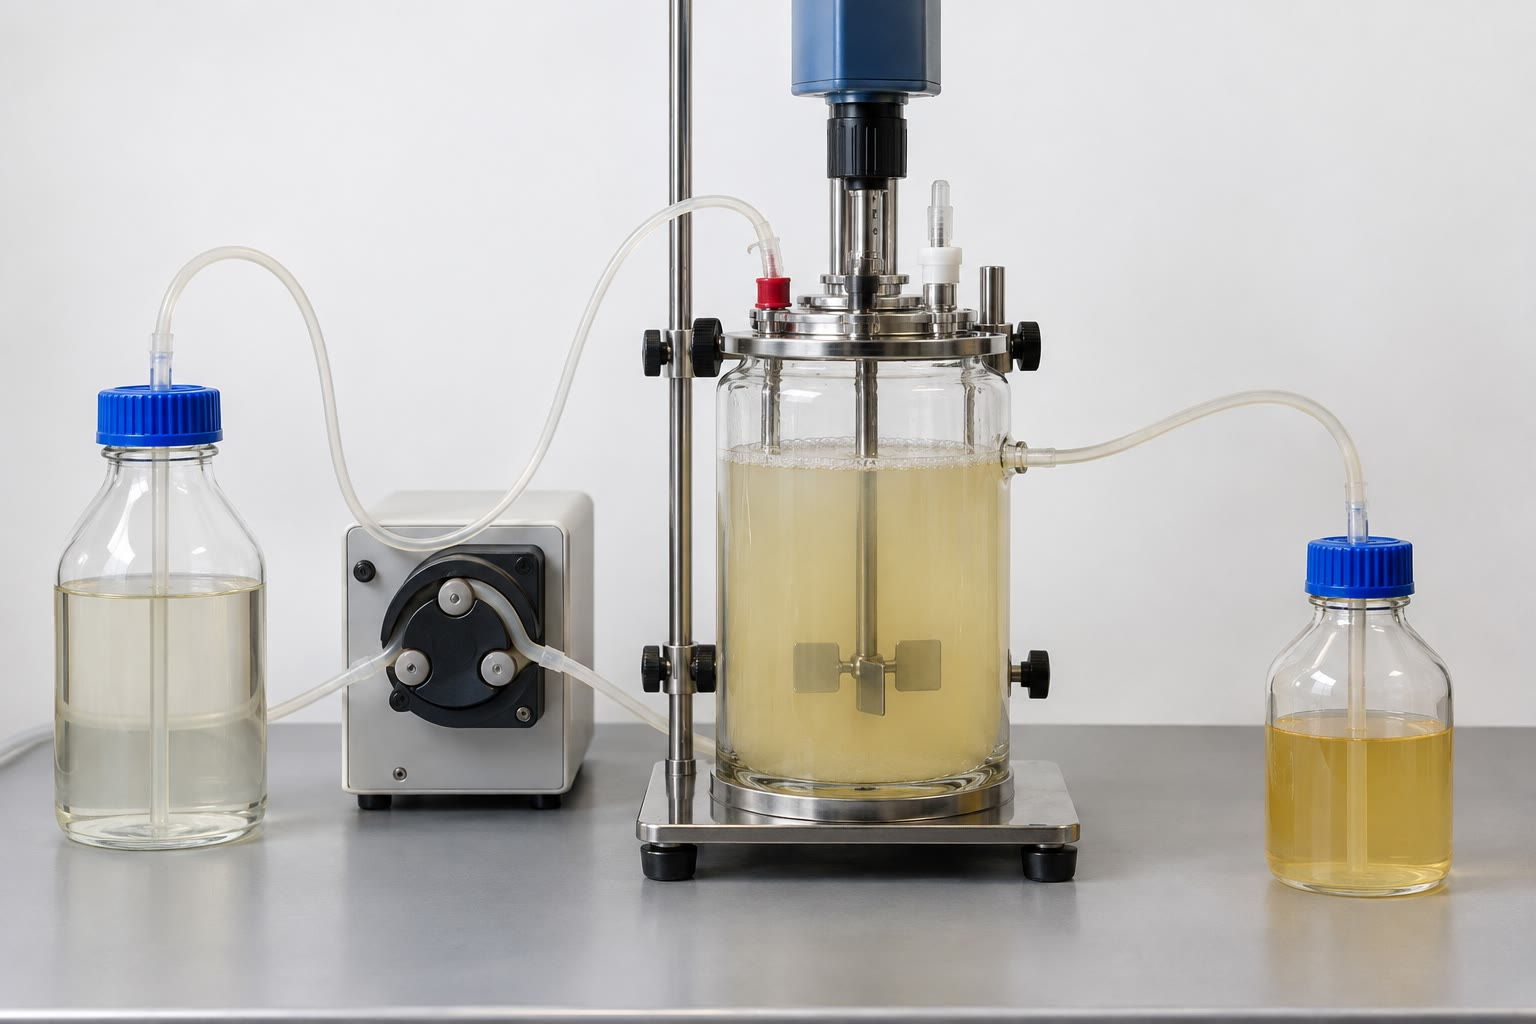
\includegraphics[width=0.6\linewidth]{images/book4/ai/b4-02-chemostat.jpg}

{\small Un quimiostato de laboratorio: el medio fresco se bombea desde el
depósito de la izquierda y el cultivo rebosa hacia la derecha; la bomba
fija la tasa de crecimiento.}
\end{omfigure}

\begin{example}[Leer un quimiostato]\label{ex:b2:microbial-metabolism:chemostat}
Con $\mu_{\max} = \qty{1.0}{h^{-1}}$, $K_s = \qty{0.02}{g/L}$,
$S_{\text{ent}} = \qty{2}{g/L}$ e $Y = 0.5$, a $D =
\qty{0.5}{h^{-1}}$: $S^* = 0.02\times 0.5/0.5 = \qty{0.02}{g/L}$ y
$X^* = 0.5\times 1.98 = \qty{0.99}{g/L}$; el cultivo deja sin usar el
\qty{1}{\%} del azúcar. La tasa de lavado es $1.0\times
2/2.02 = \qty{0.99}{h^{-1}}$. Un digestor o un intestino funcionan según
el mismo principio: el colon humano, alimentado tres veces al día y
vaciado una, mantiene sus bacterias a una \omterm{thm:b2:microbial-metabolism:chemostat}{tasa de dilución} cercana a
\qty{0.04}{h^{-1}}, y toda especie incapaz de duplicarse en un día es
eliminada por lavado --- salvo que se aferre a la pared.
\end{example}

\section{Biopelículas}

\begin{definition}[Biopelícula]\label{def:b2:microbial-metabolism:biofilm}
\index{biopelícula}\index{matriz extracelular!bacteriana}
Una \emph{biopelícula} es una comunidad de microorganismos adheridos a
una superficie e inmersos en una \emph{matriz} de polisacáridos,
proteínas y ADN extracelular que ellos mismos producen. Se forma por
etapas: \emph{adhesión} reversible de células aisladas (flagelos,
pili), adhesión irreversible y crecimiento en \emph{microcolonias},
\emph{maduración} en una película estructurada con torres y canales de
agua, y \emph{dispersión} de células que se alejan nadando para
colonizar nuevas superficies. La matriz retiene agua y nutrientes,
protege a las células de la desecación, de los consumidores, de los
antibióticos y de las células inmunitarias, y crea gradientes químicos
que hacen de la película un paisaje de nichos. La mayoría de las
bacterias de la Tierra vive así: sobre las rocas de los arroyos, en las
raíces, en los dientes (la placa dental), en catéteres e implantes, en
los pulmones de los enfermos de fibrosis quística, en los cascos de los
barcos y en las tuberías.
\end{definition}

\begin{omfigure}
\begin{tikzpicture}[every node/.style={font=\scriptsize}]
  \fill[gray!35] (0,0) rectangle (13.6,0.35);
  \node at (6.8,0.17) {superficie};
  % stage 1 attachment
  \foreach \p in {(0.6,0.55),(1.4,0.55)} \draw[thick, omDef, fill=omDef!30] \p ellipse (0.22 and 0.1);
  \draw[thick, omDef, fill=omDef!30] (1.0,1.6) ellipse (0.22 and 0.1);
  \draw[->, omDef] (1.0,1.45) -- (1.0,0.75);
  \node[below, align=center] at (1.1,-0.05) {1. adhesión};
  % stage 2 microcolony
  \begin{scope}[xshift=3.4cm]
    \fill[omExo!25] (0.15,0.35) .. controls (0.1,1.1) and (1.5,1.1) .. (1.45,0.35);
    \foreach \p in {(0.45,0.5),(0.8,0.5),(1.15,0.5),(0.6,0.75),(0.95,0.75),(0.8,0.95)} \draw[thick, omDef, fill=omDef!30] \p ellipse (0.18 and 0.09);
    \node[below, align=center] at (0.8,-0.05) {2. microcolonia,\\secreción de matriz};
  \end{scope}
  % stage 3 mature with channels
  \begin{scope}[xshift=6.8cm]
    \fill[omExo!25] (0.0,0.35) .. controls (0.2,1.9) and (0.9,2.2) .. (1.1,1.5) .. controls (1.2,0.9) and (1.4,0.6) .. (1.5,0.35);
    \fill[omExo!25] (1.7,0.35) .. controls (1.6,1.5) and (2.6,2.3) .. (2.9,1.2) .. controls (3.0,0.8) and (3.1,0.5) .. (3.2,0.35);
    \foreach \p in {(0.35,0.55),(0.7,0.55),(0.5,0.85),(0.8,1.15),(0.55,1.45),(2.0,0.6),(2.4,0.6),(2.2,0.9),(2.5,1.25),(2.3,1.6),(2.6,1.9),(2.1,1.3)} \draw[thick, omDef, fill=omDef!30] \p ellipse (0.16 and 0.08);
    \draw[<->, omThm, thick] (1.6,0.5) -- (1.6,1.6);
    \node[omThm, anchor=south] at (1.6,2.45) {canal de agua};
    \node[below, align=center] at (1.6,-0.05) {3. película madura: torres,\\canales, gradientes};
  \end{scope}
  % stage 4 dispersal
  \begin{scope}[xshift=11.2cm]
    \fill[omExo!25] (0.0,0.35) .. controls (0.1,1.5) and (1.0,1.6) .. (1.1,0.35);
    \foreach \p in {(0.3,0.55),(0.65,0.55),(0.5,0.85)} \draw[thick, omDef, fill=omDef!30] \p ellipse (0.16 and 0.08);
    \foreach \p/\a in {(1.4,1.5)/40,(1.9,1.1)/10,(1.6,2.0)/70} \draw[thick, omDef, fill=omDef!30, rotate around={\a:\p}] \p ellipse (0.16 and 0.08);
    \draw[->, omDef] (1.0,1.0) -- (1.35,1.35);
    \node[below, align=center] at (1.0,-0.05) {4. dispersión};
  \end{scope}
\end{tikzpicture}

{\small El ciclo de vida de una \omterm{def:b2:microbial-metabolism:biofilm}{biopelícula}: las células aisladas se
adhieren, crecen en microcolonias que secretan una matriz (gris), maduran
en una película estructurada con torres y canales de agua, y liberan
células nadadoras que colonizan nuevas superficies.}
\end{omfigure}

\begin{omfigure}
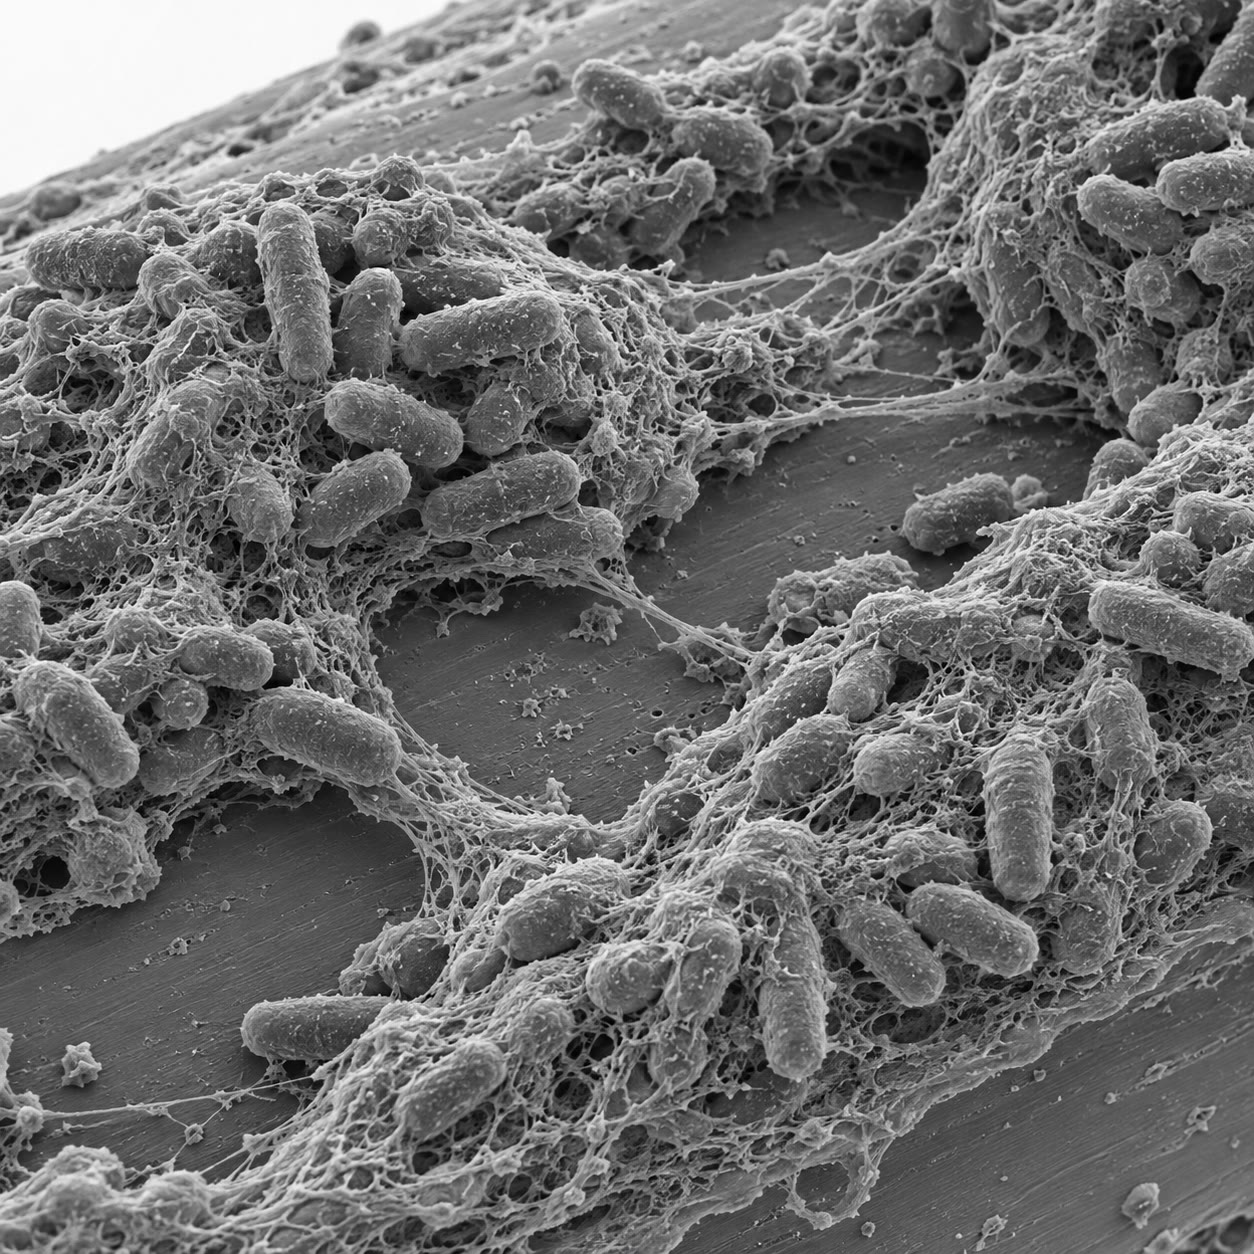
\includegraphics[width=0.46\linewidth]{images/book4/ai/b4-02-biofilm-sem.jpg}

{\small Una \omterm{def:b2:microbial-metabolism:biofilm}{biopelícula} sobre un catéter, vista al microscopio
electrónico de barrido: bacterias en forma de bastón inmersas en la
matriz fibrosa que han secretado, con canales abiertos entre los
agregados.}
\end{omfigure}

\begin{theorem}[Gradientes en el interior de una biopelícula]\label{thm:b2:microbial-metabolism:gradient}
\index{profundidad de penetración del oxígeno}
En una película de espesor $L$ cuyas células consumen oxígeno a una tasa
volumétrica constante $q$, con la concentración mantenida en $c_0$ en la
superficie y sin flujo a través del sustrato de apoyo, el perfil de
oxígeno en estado estacionario es una parábola y, si la película es lo
bastante gruesa para que el oxígeno se agote, este se agota a la
\emph{profundidad de penetración}
\[
L_p = \sqrt{\frac{2 D_e\, c_0}{q}},
\]
donde $D_e$ es el coeficiente de difusión efectivo en la matriz.
Con $D_e = \qty{1.5e-9}{m^2/s}$, $c_0 = \qty{0.25}{mol/m^3}$ y $q
= \qty{0.17}{mol/m^3/s}$ (una película densa de células que respiran), $L_p
\approx \qty{66}{\micro m}$: por debajo de una décima de milímetro una
\omterm{def:b2:microbial-metabolism:biofilm}{biopelícula} es anóxica, y las desnitrificantes, los fermentadores y las
reductoras del sulfato viven bajo un techo de aerobios.
\end{theorem}
\begin{proof}
Sea $x$ la profundidad bajo la superficie. En estado estacionario el
flujo difusivo $-D_e\,\mathrm{d}c/\mathrm{d}x$ solo varía con la
profundidad por el consumo: $D_e\,\mathrm{d}^2c/\mathrm{d}x^2 = q$.
Integrando dos veces, $c = c_0 + a x + q x^2/2D_e$. Si el oxígeno se anula
a la profundidad $L_p$ con flujo nulo en ese punto (no llega nada desde
abajo), $c(L_p) = 0$ y $c'(L_p) = 0$: la segunda da $a = -qL_p/D_e$,
y la primera da entonces $c_0 - qL_p^2/D_e + qL_p^2/2D_e = 0$, es decir,
$L_p^2 = 2D_e c_0/q$. El perfil es $c = (q/2D_e)(L_p - x)^2$.
\end{proof}

\begin{omfigure}
\begin{tikzpicture}
\begin{axis}[
  width=0.78\linewidth, height=5.6cm,
  axis x line=bottom, axis y line=left,
  xmin=0, xmax=120, ymin=0, ymax=0.28,
  xlabel={profundidad en la película (\unit{\micro m})}, ylabel={$\mathrm{O_2}$ (\unit{mol/m^3})},
  xlabel style={font=\small, at={(axis description cs:0.5,-0.14)}, anchor=north},
  ylabel style={font=\small},
  tick label style={font=\small}, xtick={0,20,40,60,80,100,120}, ytick={0,0.1,0.2},
  clip=false,
]
\addplot[very thick, omDef, domain=0:66, samples=60] {0.25*(1-x/66)^2};
\addplot[very thick, omDef, domain=66:120, samples=2] {0};
\fill[omThm!12] (axis cs:66,0) rectangle (axis cs:120,0.28);
\node[font=\scriptsize, anchor=north, align=center] at (axis cs:93,0.27) {zona anóxica:\\desnitrificantes, fermentadores,\\reductoras del sulfato};
\draw[dashed, gray] (axis cs:66,0) -- (axis cs:66,0.28); \node[font=\scriptsize, anchor=south] at (axis cs:66,0.28) {$L_p$};
\node[font=\scriptsize, anchor=west] at (axis cs:24,0.18) {zona aerobia};
\end{axis}
\end{tikzpicture}

{\small El oxígeno en el interior de una \omterm{def:b2:microbial-metabolism:biofilm}{biopelícula} que respira: una
caída parabólica desde el valor del medio en la superficie hasta cero en
la profundidad de penetración, \qty{66}{\micro m} para las cifras del
teorema. Todo lo que queda más abajo es anóxico.}
\end{omfigure}

\begin{proposition}[Percepción de quórum]\label{prop:b2:microbial-metabolism:quorum}
\index{percepción de quórum}\index{autoinductor}
Las bacterias se cuentan. Cada célula secreta, a un ritmo bajo y
constante, una pequeña molécula señal, un \emph{autoinductor}
(acil-homoserina lactonas en las gramnegativas, péptidos cortos en las
grampositivas). En una suspensión diluida la señal se dispersa por
difusión; en una población densa o en una \omterm{def:b2:microbial-metabolism:biofilm}{biopelícula} se acumula y, por
encima de una concentración umbral, se une a un receptor que activa un
conjunto de genes --- entre ellos el del propio autoinductor, de ahí el
nombre. Los genes así controlados son los que solo resultan rentables
cuando muchas células actúan a la vez: la luminiscencia, la secreción de
enzimas digestivas y de toxinas, la producción de matriz, la virulencia
de los patógenos que deben desbordar al hospedador de golpe en vez de
alertarlo célula a célula.
\end{proposition}
\begin{proof}[Evidencia]
Nealson, Platt y Hastings (1970) descubrieron que la bacteria marina
\emph{Vibrio fischeri}, que ilumina el órgano de un calamar, permanece
oscura en cultivo diluido y solo brilla por encima de unas $10^{7}$
células por mililitro; el medio sin células tomado de un cultivo denso y
luminoso hacía brillar al instante uno diluido. El medio contenía la
señal; su estructura, una acil-homoserina lactona, se determinó en 1981,
y los mutantes incapaces de fabricarla nunca brillan, por densos que
lleguen a ser.
\end{proof}

\begin{example}[Por qué una biopelícula sobrevive a los antibióticos]\label{ex:b2:microbial-metabolism:tolerance}
Las células de una \omterm{def:b2:microbial-metabolism:biofilm}{biopelícula} sobreviven a concentraciones de
antibiótico de cien a mil veces superiores a las que matan a la misma
cepa en suspensión, sin gen de resistencia alguno. La matriz frena la
difusión del fármaco y fija una parte; los gradientes dejan a las células
profundas hambrientas, anóxicas y casi sin crecer, y la mayoría de los
antibióticos solo matan células en crecimiento (las penicilinas
necesitan la síntesis de la pared; los aminoglucósidos, el transporte
activo); unas pocas células \emph{persistentes} están en completa
latencia y regeneran la película cuando se interrumpe el tratamiento.
Por eso una infección crónica sobre un implante suele tratarse
retirando el implante.
\end{example}

\section{Comunidades microbianas}

\begin{example}[La columna de Winogradsky, explicada]\label{ex:b2:microbial-metabolism:column}
La luz y el aire entran por arriba; la materia orgánica y el sulfato,
desde el barro. Las cianobacterias y las algas crecen en la parte
superior y liberan oxígeno. Debajo, los heterótrofos agotan el oxígeno
sobre la materia orgánica, y después el nitrato; más abajo, las
reductoras del sulfato transforman el sulfato en sulfuro, que difunde
hacia arriba y ennegrece el barro con sulfuro de hierro. Donde el sulfuro
ascendente se encuentra con la luz descendente, las bacterias púrpuras
del azufre lo oxidan por fotosíntesis (la banda púrpura), y las verdes
del azufre, debajo de ellas; donde el sulfuro se encuentra con el
oxígeno, en la oscuridad, oxidantes incoloras del azufre como
\emph{Beggiatoa} se ganan la vida por \omterm{def:b2:microbial-metabolism:trophic}{quimiolitotrofia} (el velo blanco);
donde el hierro reducido se encuentra con el oxígeno, las oxidantes del
hierro dejan una banda herrumbrosa. El azufre circula entre sulfuro y
sulfato dentro de la columna; el carbono, entre el $\mathrm{CO_2}$ y la
materia orgánica; solo entra la luz y solo sale el calor. Es un
ecosistema cerrado con un balance de energía abierto, y una maqueta del
fondo oceánico.
\end{example}

\begin{omfigure}
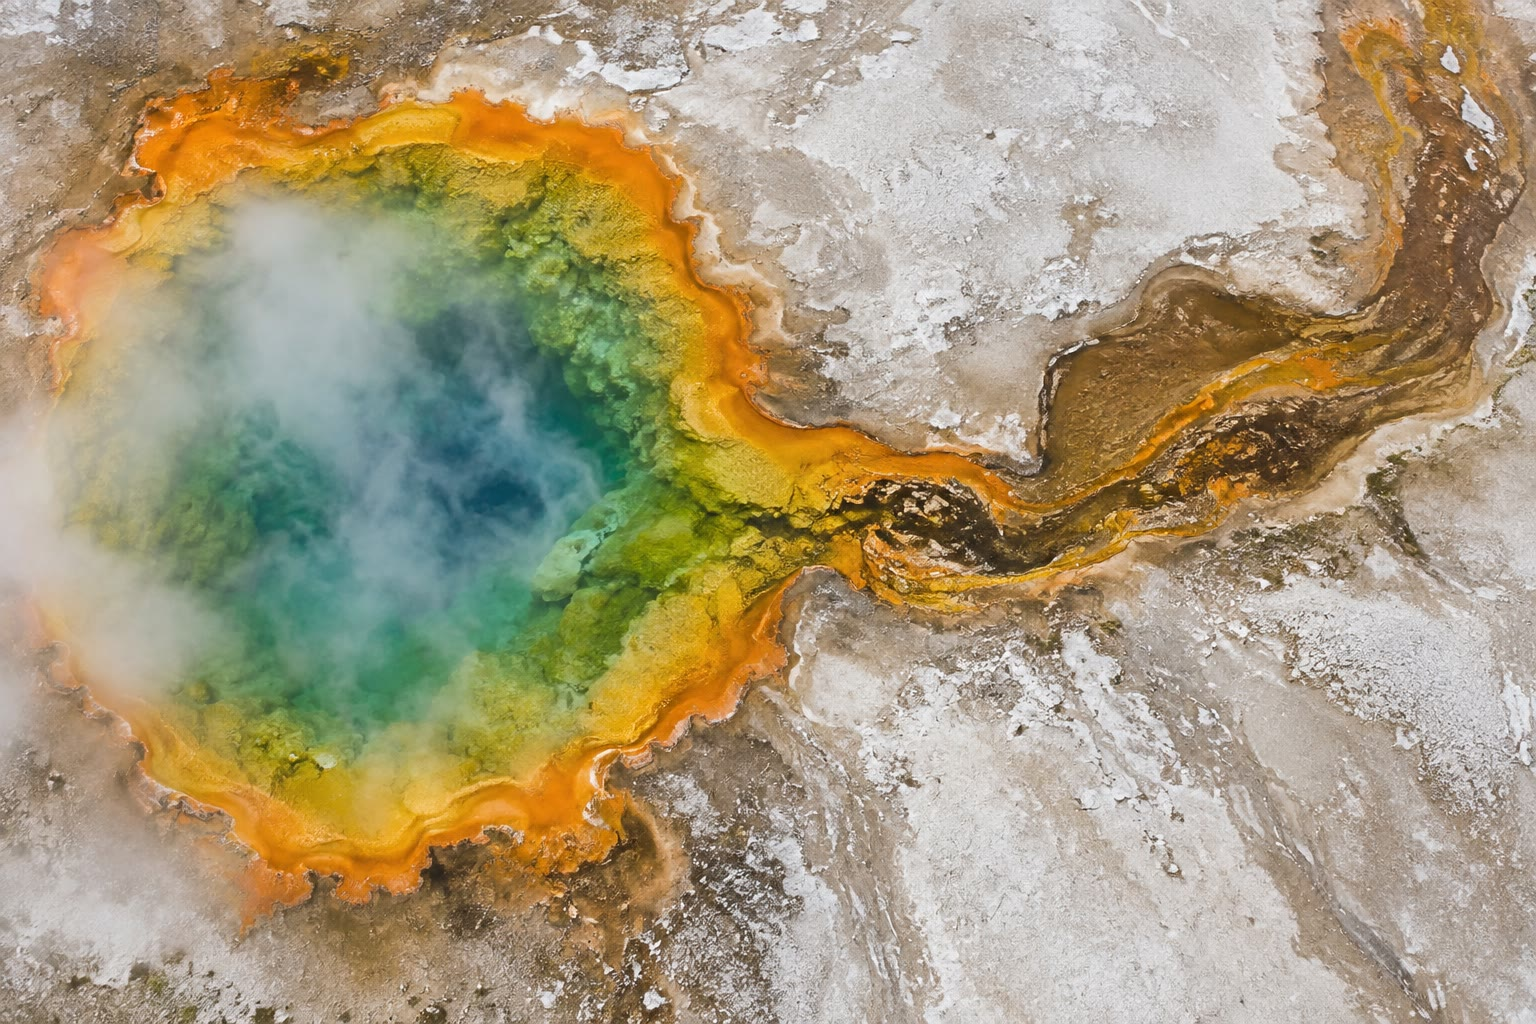
\includegraphics[width=0.62\linewidth]{images/book4/ai/b4-02-hot-spring-mats.jpg}

{\small Tapetes microbianos alrededor de una fuente termal: cada color es
una población que vive a la temperatura y con la química de su banda ---
cianobacterias y bacterias verdes termófilas en el agua de salida, más
fría, y \omterm{def:b2:microbial-metabolism:trophic}{quimiolitótrofos} incoloros en el agua más caliente.}
\end{omfigure}

\begin{remark}[Los tapetes microbianos y la Tierra primitiva]\label{rem:b2:microbial-metabolism:mats}
Alrededor de las fuentes termales y en las llanuras mareales, tapetes
microbianos estratificados de unos pocos milímetros de espesor
condensan toda la columna en un grosor que la luz puede atravesar:
cianobacterias arriba, bacterias púrpuras debajo, reductoras del sulfato
en la base, cada capa consumiendo lo que produce la de encima, y el
tapete migrando hacia arriba a través del sedimento que atrapa. Los
tapetes fósiles --- los estromatolitos --- son la prueba de vida más
antigua, de \num{3.5} miles de millones de años. Durante dos mil millones
de años, antes de las plantas y los animales, la biosfera fue estos
tapetes y el plancton que había sobre ellos, y fueron ellos quienes
llenaron el aire de oxígeno (\cref{ch:b2:biogeochemical-cycles}).
\end{remark}

\section{Ejercicios}
\section{Ejercicios}

\begin{exercise}[$\star$]\label{exo:b2:microbial-metabolism:1}
Clasifíquense según su fuente de energía, de electrones y de carbono: una
cianobacteria; \emph{Nitrosomonas}; \emph{E.~coli} sobre glucosa; una
bacteria púrpura no del azufre que crece a la luz sobre succinato;
\emph{Thiobacillus} sobre $\mathrm{H_2S}$ en la oscuridad.
\end{exercise}

\begin{exercise}[$\star$]\label{exo:b2:microbial-metabolism:2}
Enumérense los aceptores de electrones de la respiración por orden
decreciente de rendimiento energético, y dígase en qué parte de un
sedimento se usa cada uno.
\end{exercise}

\begin{exercise}[$\star$]\label{exo:b2:microbial-metabolism:3}
Ajústese la oxidación de la glucosa a $\mathrm{CO_2}$ por nitrato
reducido a $\mathrm{N_2}$ (en disolución ácida, con agua como otro
producto). ¿Cuántos iones nitrato hacen falta por glucosa?
\end{exercise}

\begin{exercise}[$\star$]\label{exo:b2:microbial-metabolism:4}
Defínase una \omterm{def:b2:microbial-metabolism:biofilm}{biopelícula} y nómbrense sus cuatro etapas. Dense tres
lugares donde las \omterm{def:b2:microbial-metabolism:biofilm}{biopelículas} tienen importancia para la salud humana o
la industria.
\end{exercise}

\begin{exercise}[$\star\star$]\label{exo:b2:microbial-metabolism:5}
Calcúlese $\Delta G^{\circ\prime}$ de $4\mathrm{H_2} + \mathrm{CO_2}
\to \mathrm{CH_4} + 2\mathrm{H_2O}$ a partir de los potenciales
$\mathrm{2H^+/H_2}$ (\qty{-0.42}{V}) y $\mathrm{CO_2/CH_4}$
(\qty{-0.24}{V}). ¿Cuántos ATP (a \qty{50}{kJ/mol}) puede fabricar como
máximo un metanógeno por $\mathrm{H_2}$? Coméntese su tasa de
crecimiento.
\end{exercise}

\begin{exercise}[$\star\star$]\label{exo:b2:microbial-metabolism:6}
Una bacteria tiene $\mu_{\max} = \qty{1.2}{h^{-1}}$ y $K_s =
\qty{5}{mg/L}$ de glucosa. Calcúlense $\mu$ y el \omterm{def:b2:unicellular-diversity:division}{tiempo de generación} a
1, 5 y \qty{50}{mg/L}. ¿A qué concentración crece al \qty{90}{\%} de su
máximo?
\end{exercise}

\begin{exercise}[$\star\star$]\label{exo:b2:microbial-metabolism:7}
Un quimiostato con $\mu_{\max} = \qty{0.8}{h^{-1}}$, $K_s =
\qty{0.05}{g/L}$, $S_{\text{ent}} = \qty{5}{g/L}$ e $Y = 0.4$ funciona a
$D = \qty{0.4}{h^{-1}}$. Calcúlense $S^*$, $X^*$, la producción de
biomasa por litro y por hora, y la tasa de lavado.
\end{exercise}

\begin{exercise}[$\star\star$]\label{exo:b2:microbial-metabolism:8}
Oxidar un $\mathrm{NH_4^+}$ a nitrito rinde \qty{275}{kJ}; una
nitrificante captura una cuarta parte en forma de ATP (\qty{50}{kJ/mol}),
y fijar un $\mathrm{CO_2}$ en biomasa cuesta el equivalente de 12
ATP. ¿Cuántos iones amonio debe oxidar por carbono fijado? ¿Por qué es
tan bajo el rendimiento de una nitrificante comparado con el de un
heterótrofo?
\end{exercise}

\begin{exercise}[$\star\star$]\label{exo:b2:microbial-metabolism:9}
Calcúlese la \omterm{thm:b2:microbial-metabolism:gradient}{profundidad de penetración del oxígeno} en una \omterm{def:b2:microbial-metabolism:biofilm}{biopelícula}
con $D_e =
\qty{1.2e-9}{m^2/s}$, $c_0 = \qty{0.20}{mol/m^3}$ y $q =
\qty{0.5}{mol/m^3/s}$. ¿Qué le ocurre a $L_p$ si se duplica el oxígeno
del medio? ¿Y si las células respiran cuatro veces más deprisa?
\end{exercise}

\begin{exercise}[$\star\star\star$]\label{exo:b2:microbial-metabolism:10}
Predíganse las bandas de una columna de Winogradsky de arriba abajo,
nombrando el metabolismo de cada una, y explíquese (a) por qué la banda
púrpura se forma donde se forma, (b) por qué el barro se vuelve negro,
(c) en qué sentido la columna es un sistema cerrado y en qué sentido uno
abierto.
\end{exercise}

\begin{exercise}[$\star\star\star$]\label{exo:b2:microbial-metabolism:11}
Cada célula de una población de densidad $n$ (células por litro) secreta
un autoinductor a razón de $p = 5$ moléculas por segundo; la molécula se
degrada con una constante $k = \qty{5e-4}{s^{-1}}$. Escríbase la
concentración estacionaria $A^*$ en función de $n$. El receptor se activa
a $A_c = \qty{10}{nmol/L}$: calcúlese la densidad umbral en células
por mililitro. Compárese con un cultivo denso ($10^{9}$ por
mililitro) y con el agua de mar ($10^{5}$ por mililitro), y explíquese
por qué una \omterm{def:b2:microbial-metabolism:biofilm}{biopelícula} alcanza el quórum en un volumen en el que una
suspensión nunca lo alcanzaría.
\end{exercise}

\begin{exercise}[$\star\star\star$]\label{exo:b2:microbial-metabolism:12}
``Los \omterm{def:b2:unicellular-diversity:prokaryote}{procariotas} gobiernan la química del planeta.'' Discútase a partir
de tres procesos de este capítulo que ningún eucariota puede realizar,
indicando para cada uno qué le ocurriría a la biosfera si se detuviera.
\end{exercise}

\section{Problema: una depuradora de aguas residuales}

\begin{problem}[{Problema de fin de semana --- la depuradora de una
ciudad analizada como un conjunto de reactores microbianos, desde la
energética de sus bacterias hasta el metano que la alimenta, para
terminar con el balance energético de la planta}]
\label{pb:b2:microbial-metabolism:1}
Una planta trata $Q = \qty{10000}{m^3}$ de aguas residuales al día, con
\qty{300}{g/m^3} de materia orgánica, medida como el oxígeno necesario
para quemarla (su \emph{demanda química de oxígeno}, DQO), y
\qty{40}{g/m^3} de nitrógeno amoniacal. Dispone de un tanque aireado de
fangos activados, un tanque anóxico para la \omterm{def:b2:microbial-metabolism:anaerobic}{desnitrificación} y un
digestor anaerobio para los fangos. Datos: los heterótrofos aerobios
transforman la materia orgánica con un rendimiento $Y = 0.4$ (kilogramo de
DQO de biomasa por kilogramo de DQO de sustrato, de modo que el resto se
oxida); la nitrificación necesita \qty{4.57}{kg} de $\mathrm{O_2}$ por
kilogramo de nitrógeno; la \omterm{def:b2:microbial-metabolism:anaerobic}{desnitrificación} necesita \qty{2.86}{kg} de
DQO de sustrato por kilogramo de nitrógeno nítrico; la aireación aporta
\qty{2}{kg} de $\mathrm{O_2}$ por kilovatio hora; en el digestor el
\qty{60}{\%} de la DQO de los fangos se convierte en metano, y cada
kilogramo de DQO convertido da \qty{0.35}{m^3} de metano de contenido
energético \qty{36}{MJ/m^3}, que se quema en un generador de
\qty{35}{\%} de rendimiento eléctrico. Nitrificantes:
$\mu_{\max} = \qty{0.5}{d^{-1}}$, $K_s =
\qty{1}{g/m^3}$ de nitrógeno
amoniacal.

\medskip
\noindent\textbf{Parte I --- La energética.}
\begin{enumerate}
  \item Con la \omterm{thm:b2:microbial-metabolism:redox}{torre de electrones}, calcúlese $\Delta G^{\circ\prime}$
        para la oxidación de un mol de glucosa (24 electrones a
        \qty{-0.43}{V}) por el oxígeno (\qty{+0.82}{V}).
  \item Calcúlese para el nitrato reducido a $\mathrm{N_2}$
        (\qty{+0.74}{V}) y para el sulfato reducido a sulfuro
        (\qty{-0.22}{V}).
  \item ¿Por qué la \omterm{def:b2:microbial-metabolism:anaerobic}{desnitrificación} solo empieza en el tanque anóxico, y
        por qué la \omterm{def:b2:microbial-metabolism:anaerobic}{reducción del sulfato} (con su olor) es señal de una
        planta mal gestionada?
  \item Si las células capturan el \qty{40}{\%} de la energía libre en
        forma de ATP (\qty{50}{kJ/mol}), ¿cuántos ATP por glucosa da cada
        uno de los tres metabolismos?
  \item ¿Cuánta más glucosa que un aerobio debe procesar una reductora
        del sulfato para el mismo crecimiento?
  \item Los fermentadores del digestor obtienen 2 ATP por glucosa.
        Explíquese por qué el digestor produce aun así casi nada de
        biomasa y sobre todo gas.
\end{enumerate}

\medskip
\noindent\textbf{Parte II --- El tanque aireado.}
\begin{enumerate}[resume]
  \item Calcúlese la carga diaria de materia orgánica, en kilogramos de
        DQO.
  \item Calcúlense la biomasa producida al día (como DQO) y el oxígeno
        necesario para oxidar el resto.
  \item Calcúlese la energía de aireación para la materia orgánica, en
        kilovatios hora al día.
  \item Calcúlense la carga diaria de nitrógeno y el oxígeno necesario
        para nitrificarla.
  \item Los fangos permanecen en el tanque un tiempo medio $\theta$ (el
        inverso de su \omterm{thm:b2:microbial-metabolism:chemostat}{tasa de dilución}). ¿Por debajo de qué $\theta$ son
        eliminadas por lavado las nitrificantes a cualquier concentración
        de amonio?
  \item Con $\theta = \qty{10}{d}$, calcúlese la concentración de amonio
        residual en el efluente.
  \item El invierno reduce $\mu_{\max}$ a \qty{0.25}{d^{-1}}. Vuélvase a
        calcular el amonio residual y dígase qué debe hacer el operador.
\end{enumerate}

\medskip
\noindent\textbf{Parte III --- La \omterm{def:b2:microbial-metabolism:anaerobic}{desnitrificación} y el digestor.}
El nitrato fabricado en el tanque aireado se recircula al tanque anóxico,
donde los heterótrofos lo reducen con la materia orgánica entrante.
\begin{enumerate}[resume]
  \item Calcúlese la materia orgánica (kilogramos de DQO al día)
        consumida al desnitrificar todo el nitrógeno.
  \item Calcúlense la masa de nitrógeno liberada al aire como
        $\mathrm{N_2}$ al día y la masa que sale en el efluente como
        amonio (pregunta 12), en fracción de la carga.
  \item Esa materia orgánica ya no necesita aireación. Calcúlense el
        oxígeno ahorrado y la demanda total de oxígeno de la planta
        (materia orgánica restante más nitrificación).
  \item Los fangos producidos (pregunta 8, contabilizados como DQO) van
        al digestor. Calcúlese el metano producido al día.
  \item Calcúlense la energía de ese metano y la electricidad que
        proporciona.
  \item Calcúlese la electricidad de aireación para la demanda total de
        oxígeno de la pregunta 16, y compárese.
\end{enumerate}

\medskip
\noindent\textbf{Parte IV --- El reactor de \omterm{def:b2:microbial-metabolism:biofilm}{biopelícula}.}
Un filtro percolador cultiva una \omterm{def:b2:microbial-metabolism:biofilm}{biopelícula} sobre piedras; el agua
contiene \qty{0.2}{mol/m^3} de oxígeno, $D_e = \qty{1.5e-9}{m^2/s}$, y
la película respira a $q = \qty{0.3}{mol/m^3/s}$.
\begin{enumerate}[resume]
  \item Dedúzcase el perfil de oxígeno $c(x)$ en una película lo bastante
        gruesa para volverse anóxica.
  \item Calcúlese la profundidad de penetración.
  \item La película tiene \qty{300}{\micro m} de espesor. ¿Qué fracción de
        ella es aerobia, y qué hacen las células de más abajo con el
        nitrato que difunde desde la capa aerobia?
  \item Explíquese por qué una sola \omterm{def:b2:microbial-metabolism:biofilm}{biopelícula} puede nitrificar y
        desnitrificar a la vez, algo que el tanque aireado no puede.
  \item Se añade cloro para desinfectar el efluente. Dense dos razones
        por las que la \omterm{def:b2:microbial-metabolism:biofilm}{biopelícula} sobrevive a una dosis que mata a las
        mismas bacterias en suspensión.
  \item Enúnciese el resultado: la demanda diaria de oxígeno de la
        planta, su producción de metano y la fracción de su electricidad
        de aireación que aporta el metano.
\end{enumerate}
\end{problem}
